\documentclass[11pt, oneside]{article}   	% use "amsart" instead of "article" for AMSLaTeX format
\usepackage{geometry}                		% See geometry.pdf to learn the layout options. There are lots.
\geometry{letterpaper}                   		% ... or a4paper or a5paper or ... 
%\geometry{landscape}                		% Activate for for rotated page geometry
%\usepackage[parfill]{parskip}    		% Activate to begin paragraphs with an empty line rather than an indent
\usepackage{graphicx}				% Use pdf, png, jpg, or eps� with pdflatex; use eps in DVI mode
								% TeX will automatically convert eps --> pdf in pdflatex		
\usepackage{amssymb}
\usepackage{amsmath}
\usepackage{parskip}
\usepackage{color}

\title{Exponential and logarithm}
%\author{The Author}
%\section{}
% \subsection*{R code}
\date{}							% Activate to display a given date or no date

\graphicspath{{/Users/telliott_admin/Dropbox/Tex/png/}}

% \begin{center} 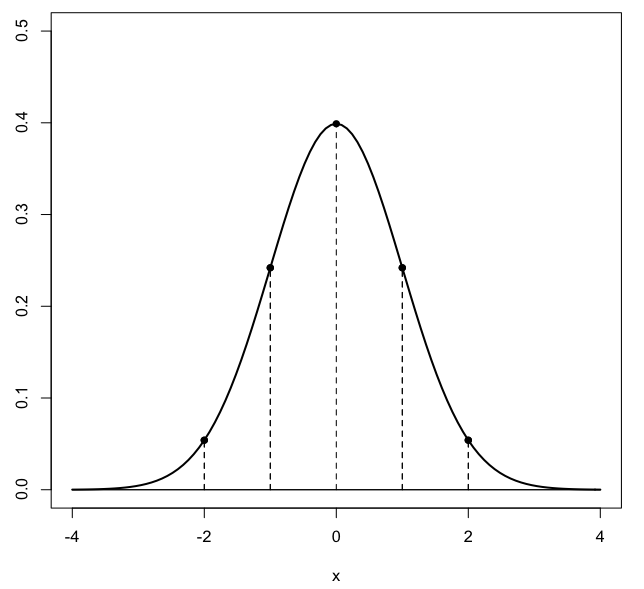
\includegraphics [scale=0.4] {gauss3.png} \end{center}
% \begin{bmatrix} a  &  b \\ c  &  d \end{bmatrix}
% \bigg |_

\begin{document}
\maketitle
\large
%\noindent

As you know, the basic idea of logarithms is that 
\[ b^p \cdot \ b^q = b^{p+q} \]
for any base $b$.  So if we know 
\[ x = b^p \]
\[ y = b^q \]
then 
\[ xy = b^{p+q} \]

and the logarithm to the base $b$ of $xy$ equals $p + q$.  To use this, we need some way of finding the number that is equal to $b^{p+q}$ (the anti-logarithm).  In the old days, tables of logarithms were used for this purpose, but today we don't bother, we use a calculator.

There is a lot of good discussion on the web about how these values were calculated.  Feynman in his \emph{Lectures on Physics} (Chapter 22 of Vol 1) has a particularly fun one.

Another fact about logarithms is the change of base formula:
\[ log_b(x) = \frac{log_a(x)}{log_a(b)} \]

We can try to remember this by noting that both terms on the right are logarithms to base $a$.  We can also check it quickly by noting that if $a < b$ then $log_a(b) > 1$ and so the factor $1/log_a(b) < 1$ so that $log_b(x) < log_a(x)$, as we expect.

\subsection*{differential calculus}

For the first part of calculus, the most important thing is that

\[ \frac{d}{dx} e^x = e^x \] 

the derivative of this function is just the function itself.
If you accept that this is a valid formula for $e^x$

\[ e^x = \frac{x^{0}}{0!} + \frac{x^{1}}{1!} + \frac{x^{2}}{2!} + \frac{x^{3}}{3!} + \cdots  = \sum_{k=0}^{\infty} \frac{x^{k}}{k!} \]

then it is easy to verify that the derivative is equal to the function, since each term $x^k/k!$ becomes  $x^{k-1}/(k-1)!$ --- except the first, which is a constant with derivative equal to $0$.

We can also use the chain rule to differentiate more complicated functions, e.g.

\[ \frac{d}{dx} e^{x^2} = 2x \ e^{x^2} \] 

Also, if 
\[ x = e^y \]
then
\[ y = log_e(x) = \ln(x) \]

We say that $y$ is the \emph{natural} logarithm of $x$.

It is worth remembering that $e$ is just a number (although a very special one).  One problem that seems tricky at first is

\[ \frac{d}{dx} 3^x = \ ? \] 

But remember that

\[ e^{ln(3)} = 3  \]
so we have
\[ 3^x = (e^{ln(3)})^x  =  e^{\ln(3) \cdot x} \]
So
\[ \frac{d}{dx} 3^x =  \frac{d}{dx} e^{\ln(3) \cdot x} = \ln(3) e^{x \ln(3)}  =  \ln(3) \cdot 3^x \] 

How about 
\[ \frac{d}{dx} \ln(x) =  \ ? \] 

Using the identity $x = e^{\ln(x)}$

\[ \frac{d}{dx} x = \frac{d}{dx} \ e^{\ln(x)} \] 

But the left-hand side is just $1$ so

\[ 1 = \frac{d}{dx} \ e^{\ln(x)} =  e^{\ln(x)} \cdot  \frac{d}{dx} \ln(x)  \] 

(again, by the chain rule).  But we can substitute back for $x$

\[ 1 = e^{\ln(x)} \cdot  \frac{d}{dx} \ln(x)  \] 
\[ = x \cdot  \frac{d}{dx} \ln(x)  \] 
\[  \frac{d}{dx} \ln(x) = \frac{1}{x}  \] 

This will become really useful when we start with integral calculus.  There are a lot of problems where the rate of change of $x$ is proportional to $x$ (bacterial growth, radioactive decay).

\[ \frac{dx}{dt} = k x \]
\[ \frac{1}{x} \ \frac{dx}{dt} = k \]

Solving such a problem involves finding a function whose derivative is equal to $1/x$

\[ \frac{d}{dt} F(x) = \frac{1}{x} \cdot  \frac{dx}{dt} \]

That function is $\ln(x)$.  We will have
\[ F(x) = \ln(x) = kt \]
\[ x = e^{kt} \]
Without too much explanation, $x$ depends also on its initial value at \emph{time-zero} ($t=0$)

\[ x = x_0 \ e^{kt} \]
Normally, we solve for $x/x_0 = 2$.  The corresponding value for $t$ is usually called $T$, the half-life or doubling time, depending on the problem type.

\[ 2 = \ e^{kT} \]
\[ \ln(2) = kT \]
\[ \frac{\ln(2)}{T} = k \]
so we can substitute back into the original equation

\[ x = x_0 \ e^{(\ln(2)/T) \  t} \]




\end{document}  